\documentclass[preview]{standalone}

\usepackage{amsmath}
\usepackage{amssymb}
\usepackage{tikz}
\usepackage{stellar}
\usepackage{definitions}
\usepackage{bettelini}

\begin{document}

\id{linearalgebra-affine-maps}
\genpage

\section{Affine maps}

\begin{snippetdefinition}{affine-map-definition}{Affine map}
    Let \(\mathcal{A}\) and \(\mathcal{B}\) be \affinespace[affine spaces]
    over the same \field \(\mathbb{F}\), with direction
    \vectorspace[vector spaces] \(V\) and \(W\), respectively. A
    \function
    \[
        \varphi\colon\mathcal{A}\fromto\mathcal{B}
    \]
    is \emph{affine} if there exist a point \(o\in\mathcal{A}\) and a
    \lineartransformation \(f\in\setoflineartransformations(V,W)\) such that
    \[
        \vec{\varphi(o)\varphi(p)}
        =
        f(\vec{op})
    \]
    for every \(p\in\mathcal{A}\).
\end{snippetdefinition}

\begin{snippet}{affine-map-origin-formula}
    After choosing an origin \(o\in\mathcal{A}\), an \affinemap behaves like
    a linear map followed by a translation:
    \[
        \varphi(p)=\varphi(o)+f(\vec{op}).
    \]
    The definition is intrinsic because the same linear map works after
    changing the chosen origin.
\end{snippet}

\begin{snippetproposition}{affine-map-origin-independence}{The base point does not matter}
    Let \(\mathcal{A}\) and \(\mathcal{B}\) be \affinespace[affine spaces]
    over the same \field \(\mathbb{F}\), with direction
    \vectorspace[vector spaces] \(V\) and \(W\). Suppose that
    \(\varphi\colon\mathcal{A}\fromto\mathcal{B}\) and
    \(f\in\setoflineartransformations(V,W)\) satisfy
    \[
        \vec{\varphi(o)\varphi(p)}=f(\vec{op})
    \]
    for some \(o\in\mathcal{A}\) and for every \(p\in\mathcal{A}\). Then,
    for every \(o'\in\mathcal{A}\) and every \(p\in\mathcal{A}\),
    \[
        \vec{\varphi(o')\varphi(p)}=f(\vec{o'p}).
    \]
\end{snippetproposition}

\begin{snippetproof}{affine-map-origin-independence-proof}{affine-map-origin-independence}{The base point does not matter}
    By the Chasles relation,
    \begin{align*}
        \vec{\varphi(o')\varphi(p)}
        &=
        \vec{\varphi(o')\varphi(o)}
        +
        \vec{\varphi(o)\varphi(p)}\\
        &=
        -\vec{\varphi(o)\varphi(o')}
        +
        \vec{\varphi(o)\varphi(p)}\\
        &=
        -f(\vec{oo'})+f(\vec{op})\\
        &=
        f(-\vec{oo'}+\vec{op})\\
        &=
        f(\vec{o'p}).
    \end{align*}
\end{snippetproof}

\begin{snippetdefinition}{affine-associated-linear-map-definition}{Associated linear map}
    Let \(\mathcal{A}\) and \(\mathcal{B}\) be \affinespace[affine spaces]
    over the same \field \(\mathbb{F}\), with direction
    \vectorspace[vector spaces] \(V\) and \(W\). If
    \[
        \varphi\colon\mathcal{A}\fromto\mathcal{B}
    \]
    is an \affinemap, its \emph{associated linear map} is the unique
    \lineartransformation
    \[
        \vec{\varphi}\colon V\fromto W
    \]
    such that
    \[
        \vec{\varphi}(\vec{op})
        =
        \vec{\varphi(o)\varphi(p)}
    \]
    for every \(o,p\in\mathcal{A}\).
\end{snippetdefinition}

\begin{snippetproposition}{affine-map-image-vectors-formula}{Image vectors under an affine map}
    Let \(\mathcal{A}\) and \(\mathcal{B}\) be \affinespace[affine spaces]
    over the same \field \(\mathbb{F}\), and let
    \[
        \varphi\colon\mathcal{A}\fromto\mathcal{B}
    \]
    be an \affinemap. Then, for every \(p,q\in\mathcal{A}\),
    \[
        \vec{\varphi(p)\varphi(q)}
        =
        \vec{\varphi}(\vec{pq}).
    \]
\end{snippetproposition}

\begin{snippetproof}{affine-map-image-vectors-formula-proof}{affine-map-image-vectors-formula}{Image vectors under an affine map}
    Fix \(o\in\mathcal{A}\). Then
    \begin{align*}
        \vec{\varphi(p)\varphi(q)}
        &=
        \vec{\varphi(p)\varphi(o)}
        +
        \vec{\varphi(o)\varphi(q)}\\
        &=
        -\vec{\varphi(o)\varphi(p)}
        +
        \vec{\varphi(o)\varphi(q)}\\
        &=
        -\vec{\varphi}(\vec{op})
        +
        \vec{\varphi}(\vec{oq})\\
        &=
        \vec{\varphi}(-\vec{op}+\vec{oq})\\
        &=
        \vec{\varphi}(\vec{pq}).
    \end{align*}
\end{snippetproof}

\section{Examples}

\begin{snippetexample}{constant-affine-map-example}{Constant maps}
    Let \(\mathcal{A}\) be an \affinespace over a \field \(\mathbb{F}\),
    and let \(\mathcal{B}=\{p\}\) be the one-point \affinespace, whose
    direction \vectorspace is \(\{0\}\). Every map
    \[
        \varphi\colon\mathcal{A}\fromto\{p\}
    \]
    is affine. Its \associatedlinearmap is the zero linear map
    \[
        \vec{\varphi}\colon V\fromto\{0\}.
    \]
\end{snippetexample}

\begin{snippetexample}{affine-line-self-maps-example}{Affine maps of the affine line}
    Let \(\mathbb{F}\) be a \field. Every \affinemap
    \[
        \varphi\colon\mathbb{A}^1(\mathbb{F})\fromto
        \mathbb{A}^1(\mathbb{F})
    \]
    has the form
    \[
        \varphi(x)=ax+b
    \]
    for some \(a,b\in\mathbb{F}\). Indeed, choosing \(0\) as base point,
    the \associatedlinearmap has the form \(x\mapsto ax\), and
    \(b=\varphi(0)\).
\end{snippetexample}

\begin{snippetexample}{vector-spaces-affine-map-example}{Affine maps between vector spaces}
    Let \(U\) and \(V\) be \vectorspace[vector spaces] over a
    \field \(\mathbb{F}\), considered as \affinespace[affine spaces] with
    their canonical affine structures. A map
    \[
        \varphi\colon U\fromto V
    \]
    is affine if and only if there exist a
    \lineartransformation \(f\in\setoflineartransformations(U,V)\) and a
    vector \(v_0\in V\) such that
    \[
        \varphi(u)=f(u)+v_0
    \]
    for every \(u\in U\).
\end{snippetexample}

\section{Translations and homotheties}

\begin{snippetdefinition}{affine-translation-definition}{Translation}
    Let \(\mathcal{A}\) be an \affinespace over a \field \(\mathbb{F}\),
    with direction \vectorspace \(V\). For \(u\in V\), the
    \emph{translation of vector \(u\)} is the map
    \[
        t_u\colon\mathcal{A}\fromto\mathcal{A}
    \]
    defined by
    \[
        \vec{pt_u(p)}=u
    \]
    for every \(p\in\mathcal{A}\).
\end{snippetdefinition}

\begin{snippetproposition}{affine-map-identity-linear-part-translation}{Translations are exactly affine maps with identity linear part}
    Let \(\mathcal{A}\) be an \affinespace over a \field \(\mathbb{F}\),
    with direction \vectorspace \(V\). An \affinemap
    \[
        \varphi\colon\mathcal{A}\fromto\mathcal{A}
    \]
    has
    \[
        \vec{\varphi}=\identityfunc_V
    \]
    if and only if \(\varphi\) is a \translationmap.
\end{snippetproposition}

\begin{snippetproof}{affine-map-identity-linear-part-translation-proof}{affine-map-identity-linear-part-translation}{Translations are exactly affine maps with identity linear part}
    If \(\vec{\varphi}=\identityfunc_V\), then for every
    \(p,q\in\mathcal{A}\),
    \[
        \vec{\varphi(p)\varphi(q)}=\vec{pq}.
    \]
    Hence all oriented segments \(\vec{p\varphi(p)}\) are equal, so
    \(\varphi\) moves every point by the same vector and is a
    \translationmap.

    Conversely, if \(\varphi=t_u\), then
    \[
        \vec{\varphi(p)\varphi(q)}=\vec{pq}
    \]
    for every \(p,q\in\mathcal{A}\), and therefore
    \(\vec{\varphi}=\identityfunc_V\).
\end{snippetproof}

\begin{snippetdefinition}{affine-homothety-definition}{Homothety}
    Let \(\mathcal{A}\) be an \affinespace over a \field \(\mathbb{F}\),
    with direction \vectorspace \(V\). Fix \(o\in\mathcal{A}\) and
    \(\lambda\in\mathbb{F}\). The \emph{homothety with center \(o\) and
    ratio \(\lambda\)} is the map
    \[
        h_{o,\lambda}\colon\mathcal{A}\fromto\mathcal{A}
    \]
    defined by
    \[
        \vec{o\,h_{o,\lambda}(p)}
        =
        \lambda\vec{op}
    \]
    for every \(p\in\mathcal{A}\).
\end{snippetdefinition}

\begin{snippetexample}{affine-homothety-plane-example}{Homotheties in the affine plane}
    If \(\lambda>1\), the \homothety expands distances from its center. If
    \(0<\lambda<1\), it contracts them. If \(\lambda=-1\), it is the
    central symmetry with center \(o\).
    \[
        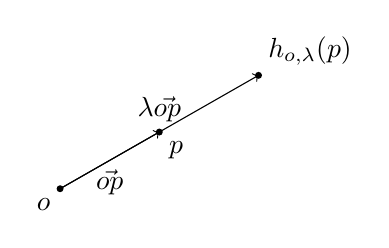
\begin{tikzpicture}[scale=0.9]
            \coordinate (O) at (0,0);
            \coordinate (P) at (1.4,0.8);
            \coordinate (H) at (2.8,1.6);

            \draw[->] (O) -- (P) node[midway, below] {\(\vec{op}\)};
            \draw[->] (O) -- (H) node[midway, above] {\(\lambda\vec{op}\)};
            \fill (O) circle (1.4pt) node[below left] {\(o\)};
            \fill (P) circle (1.4pt) node[below right] {\(p\)};
            \fill (H) circle (1.4pt) node[above right] {\(h_{o,\lambda}(p)\)};
        \end{tikzpicture}
    \]
\end{snippetexample}

\section{Composition}

\begin{snippetproposition}{affine-map-composition-and-inverse}{Composition and inverse of affine maps}
    Let \(\mathcal{A},\mathcal{B},\mathcal{C}\) be
    \affinespace[affine spaces] over a \field \(\mathbb{F}\). If
    \[
        \varphi\colon\mathcal{A}\fromto\mathcal{B},
        \qquad
        \psi\colon\mathcal{B}\fromto\mathcal{C}
    \]
    are \affinemap[affine maps], then \(\psi\circ\varphi\) is affine and
    \[
        \vec{\psi\circ\varphi}
        =
        \vec{\psi}\circ\vec{\varphi}.
    \]
    If \(\varphi\colon\mathcal{A}\fromto\mathcal{B}\) is a bijective
    \affinemap, then \(\varphi^{-1}\) is affine and
    \[
        \vec{\varphi^{-1}}
        =
        \vec{\varphi}^{-1}.
    \]
\end{snippetproposition}

\begin{snippetproof}{affine-map-composition-and-inverse-proof}{affine-map-composition-and-inverse}{Composition and inverse of affine maps}
    For \(p,q\in\mathcal{A}\),
    \begin{align*}
        \vec{(\psi\circ\varphi)(p)(\psi\circ\varphi)(q)}
        &=
        \vec{\psi(\varphi(p))\psi(\varphi(q))}\\
        &=
        \vec{\psi}\bigl(\vec{\varphi(p)\varphi(q)}\bigr)\\
        &=
        \vec{\psi}\bigl(\vec{\varphi}(\vec{pq})\bigr)\\
        &=
        (\vec{\psi}\circ\vec{\varphi})(\vec{pq}).
    \end{align*}
    Hence \(\psi\circ\varphi\) is affine with associated linear map
    \(\vec{\psi}\circ\vec{\varphi}\).

    Now suppose that \(\varphi\) is bijective. If
    \(\vec{\varphi}(u)=0\), choose \(p,q\in\mathcal{A}\) with
    \(u=\vec{pq}\). Then
    \[
        \vec{\varphi(p)\varphi(q)}=0,
    \]
    so \(\varphi(p)=\varphi(q)\), and by injectivity \(p=q\). Thus
    \(u=0\), so \(\vec{\varphi}\) is injective.

    To prove surjectivity, let \(w\) be a vector in the direction
    \vectorspace of \(\mathcal{B}\). Choose \(r,s\in\mathcal{B}\) such
    that \(w=\vec{rs}\). Since \(\varphi\) is surjective, write
    \(r=\varphi(p)\) and \(s=\varphi(q)\). Then
    \[
        w=\vec{\varphi(p)\varphi(q)}=\vec{\varphi}(\vec{pq}).
    \]
    Thus \(\vec{\varphi}\) is bijective.

    If \(r,s\in\mathcal{B}\), put \(p=\varphi^{-1}(r)\) and
    \(q=\varphi^{-1}(s)\). Then
    \[
        \vec{rs}
        =
        \vec{\varphi(p)\varphi(q)}
        =
        \vec{\varphi}(\vec{pq}),
    \]
    so
    \[
        \vec{\varphi^{-1}(r)\varphi^{-1}(s)}
        =
        \vec{pq}
        =
        \vec{\varphi}^{-1}(\vec{rs}).
    \]
    Hence \(\varphi^{-1}\) is affine and
    \(\vec{\varphi^{-1}}=\vec{\varphi}^{-1}\).
\end{snippetproof}

\begin{snippetdefinition}{affine-group-definition}{Affine group}
    Let \(\mathcal{A}\) be an \affinespace. The \emph{affine group} of
    \(\mathcal{A}\), denoted
    \[
        \affgrp(\mathcal{A}),
    \]
    is the \group of all bijective affine maps
    \[
        \varphi\colon\mathcal{A}\fromto\mathcal{A}
    \]
    under composition.
\end{snippetdefinition}

\begin{snippetproposition}{affine-group-linear-part-homomorphism}{Linear part homomorphism}
    Let \(\mathcal{A}\) be an \affinespace over a \field \(\mathbb{F}\),
    with direction \vectorspace \(V\). The map
    \[
        \affgrp(\mathcal{A})
        \fromto
        \{\text{invertible linear maps }V\fromto V\},
        \qquad
        \varphi\mapsto\vec{\varphi},
    \]
    is a \grouphomomorphism.
\end{snippetproposition}

\begin{snippetproof}{affine-group-linear-part-homomorphism-proof}{affine-group-linear-part-homomorphism}{Linear part homomorphism}
    If \(\varphi,\psi\in\affgrp(\mathcal{A})\), then
    \[
        \vec{\varphi\circ\psi}
        =
        \vec{\varphi}\circ\vec{\psi}.
    \]
    Moreover,
    \[
        \vec{\identityfunc_{\mathcal{A}}}=\identityfunc_V.
    \]
    Hence the assignment preserves composition and identity.
\end{snippetproof}

\begin{snippetproposition}{affine-group-linear-part-kernel}{Kernel of the linear part homomorphism}
    Let \(\mathcal{A}\) be an \affinespace over a \field \(\mathbb{F}\),
    with direction \vectorspace \(V\). The kernel of
    \[
        \affgrp(\mathcal{A})
        \fromto
        \{\text{invertible linear maps }V\fromto V\},
        \qquad
        \varphi\mapsto\vec{\varphi},
    \]
    is the \subgroup of translations.
\end{snippetproposition}

\begin{snippetproof}{affine-group-linear-part-kernel-proof}{affine-group-linear-part-kernel}{Kernel of the linear part homomorphism}
    The kernel consists of those \(\varphi\) with
    \[
        \vec{\varphi}=\identityfunc_V.
    \]
    By the characterization of translations, these are exactly the
    translations \(t_u\), with \(u\in V\). They form a subgroup because
    \[
        t_u\circ t_v=t_{u+v},
        \qquad
        t_0=\identityfunc_{\mathcal{A}},
        \qquad
        t_u^{-1}=t_{-u}.
    \]
\end{snippetproof}

\begin{snippetcorollary}{affine-group-decomposition-at-point}{Decomposition with respect to a point}
    Let \(\mathcal{A}\) be an \affinespace over a \field \(\mathbb{F}\),
    with direction \vectorspace \(V\). Fix \(o\in\mathcal{A}\). Every
    \[
        \varphi\in\affgrp(\mathcal{A})
    \]
    can be written uniquely as
    \[
        \varphi=t_u\circ\psi,
    \]
    where \(t_u\) is a \translationmap and
    \(\psi\in\affgrp(\mathcal{A})\) satisfies \(\psi(o)=o\).
\end{snippetcorollary}

\begin{snippetproof}{affine-group-decomposition-at-point-proof}{affine-group-decomposition-at-point}{Decomposition with respect to a point}
    Let
    \[
        u=\vec{o\varphi(o)}
    \]
    and put \(\psi=t_{-u}\circ\varphi\). Then \(\psi(o)=o\), and
    \[
        \varphi=t_u\circ\psi.
    \]
    The vector \(u\) is forced by \(u=\vec{o\varphi(o)}\), so the
    decomposition is unique.
\end{snippetproof}

\section{Coordinates}

\begin{snippetdefinition}{affine-homogeneous-coordinates-definition}{Homogeneous coordinates for affine maps}
    Let \(\mathbb{F}\) be a \field. An \affinemap in coordinates
    \[
        \widetilde{\varphi}\colon\mathbb{F}^m\fromto\mathbb{F}^n,
        \qquad
        \widetilde{\varphi}(x)=Ax+b,
    \]
    with \(A\in\matrices_{n\times m}(\mathbb{F})\) and
    \(b\in\mathbb{F}^n\), is represented in
    \emph{homogeneous coordinates} by
    \[
        \begin{pmatrix}
            A & b\\
            0 & 1
        \end{pmatrix}
        \in\matrices_{(n+1)\times(m+1)}(\mathbb{F}).
    \]
\end{snippetdefinition}

\begin{snippet}{homogeneous-coordinates-explanation}
    The point \(x=(x_1,\ldots,x_m)\) is identified with the column vector
    \[
        \begin{pmatrix}
            x_1\\
            \vdots\\
            x_m\\
            1
        \end{pmatrix}.
    \]
    Then
    \[
        \begin{pmatrix}
            A & b\\
            0 & 1
        \end{pmatrix}
        \begin{pmatrix}
            x\\
            1
        \end{pmatrix}
        =
        \begin{pmatrix}
            Ax+b\\
            1
        \end{pmatrix}.
    \]
    Thus the affine expression \(x\mapsto Ax+b\) becomes a matrix product
    after adding one coordinate.
\end{snippet}

\begin{snippetproposition}{affine-map-coordinate-form}{Coordinate form of affine maps}
    Let \(\mathcal{A}\) and \(\mathcal{B}\) be
    \affinespace[affine spaces] over a \field \(\mathbb{F}\), with
    dimensions \(m\) and \(n\). Choose an \affineframe of \(\mathcal{A}\)
    and an \affineframe of \(\mathcal{B}\). In the induced coordinates,
    every \affinemap
    \[
        \varphi\colon\mathcal{A}\fromto\mathcal{B}
    \]
    has the form
    \[
        \widetilde{\varphi}(x)=Ax+b
    \]
    for some \(A\in\matrices_{n\times m}(\mathbb{F})\) and
    \(b\in\mathbb{F}^n\).
\end{snippetproposition}

\begin{snippet}{affine-coordinate-diagram}
    Choosing affine frames identifies \(\mathcal{A}\) and \(\mathcal{B}\)
    with the canonical affine spaces \(\mathbb{A}^m(\mathbb{F})\) and
    \(\mathbb{A}^n(\mathbb{F})\). In those coordinates, an affine map is
    written as \(x\mapsto Ax+b\).
    \[
        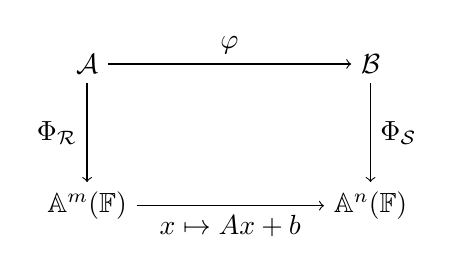
\begin{tikzpicture}[scale=0.9]
            \node (A) at (0,0) {\(\mathcal{A}\)};
            \node (B) at (4,0) {\(\mathcal{B}\)};
            \node (Fm) at (0,-2) {\(\mathbb{A}^m(\mathbb{F})\)};
            \node (Fn) at (4,-2) {\(\mathbb{A}^n(\mathbb{F})\)};

            \draw[->] (A) -- (B) node[midway, above] {\(\varphi\)};
            \draw[->] (A) -- (Fm) node[midway, left] {\(\Phi_{\mathcal{R}}\)};
            \draw[->] (B) -- (Fn) node[midway, right] {\(\Phi_{\mathcal{S}}\)};
            \draw[->] (Fm) -- (Fn) node[midway, below] {\(x\mapsto Ax+b\)};
        \end{tikzpicture}
    \]
\end{snippet}

\section{Determination}

\begin{snippetproposition}{affine-map-determined-by-affine-frame}{An affine map is determined by an affine frame}
    Let \(\mathcal{A}\) be an \(n\)-dimensional \affinespace over a
    \field \(\mathbb{F}\), and let
    \[
        \{p_0,p_1,\ldots,p_n\}
    \]
    be an \affineframe of \(\mathcal{A}\). Let
    \(\mathcal{B}\) be an \affinespace over \(\mathbb{F}\), and let
    \(q_0,\ldots,q_n\in\mathcal{B}\). Then there exists a unique
    \affinemap
    \[
        \varphi\colon\mathcal{A}\fromto\mathcal{B}
    \]
    such that
    \[
        \varphi(p_i)=q_i
    \]
    for every \(i=0,\ldots,n\).
\end{snippetproposition}

\begin{snippetproof}{affine-map-determined-by-affine-frame-proof}{affine-map-determined-by-affine-frame}{An affine map is determined by an affine frame}
    Since \(\{p_0,p_1,\ldots,p_n\}\) is an \affineframe, the vectors
    \[
        \vec{p_0p_1},\ldots,\vec{p_0p_n}
    \]
    form a \basis of the direction \vectorspace \(V\) of \(\mathcal{A}\).
    Define a \lineartransformation \(f\colon V\fromto W\) by
    \[
        f(\vec{p_0p_i})=\vec{q_0q_i}
    \]
    for \(i=1,\ldots,n\). This determines \(f\) uniquely.

    For \(p\in\mathcal{A}\), define \(\varphi(p)\) as the unique point of
    \(\mathcal{B}\) such that
    \[
        \vec{q_0\varphi(p)}=f(\vec{p_0p}).
    \]
    Then \(\varphi\) is affine and satisfies \(\varphi(p_i)=q_i\).

    If \(\psi\) is another \affinemap with \(\psi(p_i)=q_i\), then
    \[
        \vec{\psi}(\vec{p_0p_i})
        =
        \vec{\psi(p_0)\psi(p_i)}
        =
        \vec{q_0q_i}
    \]
    for every \(i=1,\ldots,n\). Hence \(\vec{\psi}=f\). Since also
    \(\psi(p_0)=q_0\), for every \(p\in\mathcal{A}\),
    \[
        \vec{q_0\psi(p)}
        =
        f(\vec{p_0p})
        =
        \vec{q_0\varphi(p)}.
    \]
    The affine-space bijection \(q\mapsto\vec{q_0q}\) gives
    \(\psi(p)=\varphi(p)\), so \(\psi=\varphi\).
\end{snippetproof}

\begin{snippetexercise}{affine-map-determined-by-three-points-exercise}{Affine map determined by three points}
    Let
    \[
        \varphi\colon\mathbb{A}^2(\realnumbers)\fromto
        \mathbb{A}^2(\realnumbers)
    \]
    be the unique \affinemap such that
    \[
        \varphi(0,0)=(-1,0),
        \qquad
        \varphi(1,1)=(-2,-1),
        \qquad
        \varphi(2,1)=(-3,-1).
    \]
    Determine \(\varphi\), its \associatedlinearmap, and its homogeneous
    coordinate \matrix.
\end{snippetexercise}

\begin{snippetsolution}{affine-map-determined-by-three-points-solution}{Affine map determined by three points}
    The three source points form an \affineframe of
    \(\mathbb{A}^2(\realnumbers)\), because the vectors
    \[
        (1,1)-(0,0)=(1,1),
        \qquad
        (2,1)-(0,0)=(2,1)
    \]
    are linearly independent.

    Write \(\varphi(x)=Ax+b\). Since \(\varphi(0,0)=(-1,0)\), we get
    \[
        b=(-1,0).
    \]
    The linear part satisfies
    \[
        A(1,1)=(-2,-1)-(-1,0)=(-1,-1),
    \]
    and
    \[
        A(2,1)=(-3,-1)-(-1,0)=(-2,-1).
    \]
    Since
    \[
        (1,0)=-(1,1)+(2,1),
        \qquad
        (0,1)=2(1,1)-(2,1),
    \]
    it follows that
    \[
        A(1,0)=(-1,0),
        \qquad
        A(0,1)=(0,-1).
    \]
    Hence \(A=-\identmatrix{2}\), and
    \[
        \varphi(x,y)=(-x-1,-y).
    \]
    In \homogeneouscoordinates, \(\varphi\) is represented by
    \[
        \begin{pmatrix}
            -1 & 0 & -1\\
            0 & -1 & 0\\
            0 & 0 & 1
        \end{pmatrix}.
    \]
\end{snippetsolution}

\end{document}
